\documentclass{agasthesis}

\usepackage{geometry}
\usepackage{pstricks}
\usepackage[latin1]{inputenc}
\usepackage[T1]{fontenc}
\usepackage{url}


\graphicspath{{images/}}
\usepackage{amsthm}
\usepackage{graphicx}


%using arcs above letters \overarc
\usepackage{arcs}

%ordentliche nummerierung
\renewcommand*{\thesection}{\arabic{section}}
%gef�llte quadrate bei proof environments 
\renewcommand{\qedsymbol}{$\blacksquare$}



\newtheorem{lemma}{Lemma}[section]
\newtheorem{prop}{Proposition}[section]
\newtheorem{definition}{Definition}[section]
%\newtheorem{theorem}{Theorem}[section]
\begin{document}
\begin{titlepage}
\enlargethispage{3em}
%%%%%%%%%%%%%%%%%%%%%%%%%%%%%%%%%%%%%%%%%%%%%%%%%%%%%%%%%%%%%%%%%
%%%%%%%%%%%%%%%%%%%%%%%%%%%%%%%%%%%%%%%%%%%%%%%%%%%%%%%%%%%%%%%%%
%%% Kopf mit Logos
\begin{minipage}{0.45\textwidth}
  \begin{flushleft} \small
    \includegraphics[width=68mm]{Uni-Logo}
    \hspace*{16mm}Fachbereich 4: Informatik
  \end{flushleft}
\end{minipage}
\hfill
\begin{minipage}{0.45\textwidth}
  \begin{flushright} \small
    % hier statt AGAS Logo ggf. Logo einer externen Org. einsetzen
    
\includegraphics[bb=0 40 706 298,height=10mm]{logo-agas-hires} \\
    % hier ggf. Namen einer externen Org. einsetzen
    {\ }
  \end{flushright}
\end{minipage}
\vfill
\hspace*{15mm}
\begin{minipage}[b]{0.8\textwidth}
  \begin{flushleft}
  \vspace{2cm}  
%%%%%%%%%%%%%%%%%%%%%%%%%%%%%%%%%%%%%%%%%%%%%%%%%%%%%%%%%%%%%%%%%
%%%%%%%%%%%%%%%%%%%%%%%%%%%%%%%%%%%%%%%%%%%%%%%%%%%%%%%%%%%%%%%%%
%%% hier den Titel der Arbeit eintragen
\LARGE{\bf Reactive Construction of Planar Euclidean Spanners with Constant Node Degree} \\
\vspace{4em}
%%%%%%%%%%%%%%%%%%%%%%%%%%%%%%%%%%%%%%%%%%%%%%%%%%%%%%%%%%%%%%%%%
%%%%%%%%%%%%%%%%%%%%%%%%%%%%%%%%%%%%%%%%%%%%%%%%%%%%%%%%%%%%%%%%%
%%% UNTERTITEL
\Large{
%%%%%%%%%%%%%%%%%%%%%%%%%%%%%%%%%%%%%%%%%%%%%%%%%%%%%%%%%%%%%%%%%
%%%%%%%%%%%%%%%%%%%%%%%%%%%%%%%%%%%%%%%%%%%%%%%%%%%%%%%%%%%%%%%%%
%%% f�r Diplomarbeit
%	Diplomarbeit \\
%	zur Erlangung des Grades \\
%	\textsc{Diplom-Informatiker} \\  % ggf. �ndern zu Diplom-Informatikerin

%%%%%%%%%%%%%%%%%%%%%%%%%%%%%%%%%%%%%%%%%%%%%%%%%%%%%%%%%%%%%%%%%
%%%%%%%%%%%%%%%%%%%%%%%%%%%%%%%%%%%%%%%%%%%%%%%%%%%%%%%%%%%%%%%%%
%%% f�r Studienarbeit
%	Studienarbeit \\

%%%%%%%%%%%%%%%%%%%%%%%%%%%%%%%%%%%%%%%%%%%%%%%%%%%%%%%%%%%%%%%%%
%%%%%%%%%%%%%%%%%%%%%%%%%%%%%%%%%%%%%%%%%%%%%%%%%%%%%%%%%%%%%%%%%
%%% f�r Masterarbeit
%	Masterarbeit \\
%	zur Erlangung des Grades\\
%	\textsc{Master of Science} \\

%%%%%%%%%%%%%%%%%%%%%%%%%%%%%%%%%%%%%%%%%%%%%%%%%%%%%%%%%%%%%%%%%
%%%%%%%%%%%%%%%%%%%%%%%%%%%%%%%%%%%%%%%%%%%%%%%%%%%%%%%%%%%%%%%%%
%%% f�r Bachelorarbeit
	Bachelorarbeit \\
	zur Erlangung des Grades\\
	\textsc{Bachelor of Science} \\
%
im Studiengang Informatik \\
} % end of \Large
%%%%%%%%%%%%%%%%%%%%%%%%%%%%%%%%%%%%%%%%%%%%%%%%%%%%%%%%%%%%%%%%%
\vspace{2em}
\small{vorgelegt von} \\
\vspace{1em}
%%%%%%%%%%%%%%%%%%%%%%%%%%%%%%%%%%%%%%%%%%%%%%%%%%%%%%%%%%%%%%%%%
%%% AUTOR
\Large{
  Tim Budweg
}
\vspace{2em}
%%%%%%%%%%%%%%%%%%%%%%%%%%%%%%%%%%%%%%%%%%%%%%%%%%%%%%%%%%%%%%%%%
%%%%%%%%%%%%%%%%%%%%%%%%%%%%%%%%%%%%%%%%%%%%%%%%%%%%%%%%%%%%%%%%%

%%%%%%%%%%%%%%%%%%%%%%%%%%%%%%%%%%%%%%%%%%%%%%%%%%%%%%%%%%%%%%%%%
%%%%%%%%%%%%%%%%%%%%%%%%%%%%%%%%%%%%%%%%%%%%%%%%%%%%%%%%%%%%%%%%%
%%% BETREUER

  \footnotesize{
      {\bf Betreuer:} M. Sc. Florentin Neumann, Institut f�r Informatik, Fachbereich Informatik, Universit�t Koblenz-Landau \\
      {\bf Erstgutachter:}   M. Sc. Florentin Neumann, Institut f�r Informatik, Fachbereich Informatik, Universit�t Koblenz-Landau \\
      {\bf Zweitgutachter:}  Prof. Dr. Hannes Frey, Institut f�r Informatik, Fachbereich Informatik, Universit�t Koblenz-Landau
    % hier Abgabemonat und -jahr eintragen
    
    \vspace{1em}
    \begin{flushleft}
    Koblenz, im 11 2015
    \end{flushleft}
 }

  \end{flushleft}
\end{minipage}

\end{titlepage}

\clearemptydoublepage
\thispagestyle{empty}
\ \vfill
\selectlanguage{german}
\section*{Kurzfassung}
Bisher existieren keine beaconlose Algorithmen, welche reaktiv einen euklidischen Spanner produzieren und zugleich konstant ausgangsgradbeschränkte Knoten beinhalten.
In dieser Bachelorarbeit werde ich untersuchen, ob die Partial Delaunay Triangulation in Verbindung mit dem Modified Yao Step einen solchen Algorithmus erzeugen kann.
Dieser Algorithmus hat im Vergleich zur derzeitigen State-Of-The-Art sowohl beim Topologieaufbau als auch beim späteren Routing über diese Topology einen verringerten Energieaufwand zur Folge, was längere Knotenlaufzeiten ermöglicht.


\selectlanguage{english}
\section*{Abstract}
Insert your abstract in english here. Lorem ipsum dolor sit amet, consectetuer adipi.
Nullam nec mi et neque pharetra sollicitudin. Praesent imperdiet mi nec ante. Donec 
ullamcorper, felis non sodales commodo, lectus velit ultrices augue, a dignissim nibh 
lectus placerat pede. Vivamus nunc nunc, molestie ut, ultricies vel, semper in, velit. 
Ut porttitor. Praesent in sapien. Lorem ipsum dolor sit amet, consectetuer adipis- 
cing elit. Duis fringilla tristique neque. Sed interdum libero ut metus. Pellentesque 
placerat. Nam rutrum augue a leo. Morbi sed elit sit amet ante lobortis sollicitudin. 
Praesent blandit blandit mauris. Praesent lec- tus tellus, aliquet aliquam, luctus a, 
egestas a, turpis. Mauris lacinia lorem sit amet ipsum. Nunc quis urna dictum turpis 
accumsan semper.
%%%%%%%%%%%%%%%%%%%%%%%%%%%%%%%%%%%%%%%%%%%%%%%%%%%%%%%%%%%%%%%%%
%%%%%%%%%%%%%%%%%%%%%%%%%%%%%%%%%%%%%%%%%%%%%%%%%%%%%%%%%%%%%%%%%
\clearemptydoublepage
\selectlanguage{german}
\subsection*{Erkl�rung}
Ich versichere, dass ich die vorliegende Arbeit selbst�ndig verfasst
und keine anderen als die angegebenen Quellen und Hilfsmittel benutzt habe
und dass die Arbeit
in gleicher oder �hnlicher Form noch keiner anderen Pr�fungsbeh�rde
vorgelegen hat und von dieser als Teil einer Pr�fungsleistung
angenommen wurde. Alle Ausf�hrungen, die w�rtlich oder sinngem��
�bernommen wurden, sind als solche gekennzeichnet.

Die Vereinbarung der Arbeitsgruppe f�r Studien- und Abschlussarbeiten
habe ich gelesen und anerkannt, insbesondere die Regelung des Nutzungsrechts.
\\[10mm]
\begin{tabular}{p{0.8\linewidth}@{\hspace*{2ex}}r@{\hspace*{2ex}}r}
Mit der Einstellung dieser Arbeit in die Bibliothek bin ich einverstanden.
& ja $\boxtimes $ & nein $\square$ \\[2em] %% change $\square$ to $\boxtimes$ to make a selection
Der Ver�ffentlichung dieser Arbeit im Internet stimme ich zu.
& ja $\boxtimes $ & nein $\square$ \\
\end{tabular}
\\[20mm]

Koblenz, den \today \\[10mm]

%%%%%%%%%%%%%%%%%%%%%%%%%%%%%%%%%%%%%%%%%%%%%%%%%%%%%%%%%%%%%%%%%
%%%%%%%%%%%%%%%%%%%%%%%%%%%%%%%%%%%%%%%%%%%%%%%%%%%%%%%%%%%%%%%%%

%% uncomment for english thesis
\selectlanguage{english}

%% TOC, LOT and LOF
\tableofcontents
\listoftables
\listoffigures

%% include your chapters here
\section{Introduction}
Wireless ad-hoc sensor networks are very useful. 
You can create warning systems for emergency purposes.
For instance, deploying many sensor nodes into the sea or forest to check and caution for tsunamis or fire, respectively.

If a node detects something and sends a message, it is obvious that this message needs to \emph{arrive} at a certain station.
The message should not get lost.
To achieve this guaranteed message delivery in a multi-hop network a specific graph-property called planarity must be satisfied.

Explaining planarity imagine a graph setup watched from above. 
It creates a 2d-view of this graph.
Planarity says that from this view no two edges are allowed to cross each other except in the endpoints.

To planarize a graph some edges must be removed.
If edges are arbitrarily removed from this graph it may result in a disconnected graph or at least randomly long paths.
This needs to be prohibited and can be achieved if a so called \emph{euclidian t-spanner} property is satisfied.
\section{Algorithm}
This chapter introduces the $reactive Modified Yao Step $ and explains it's functionality.
First, there is the basic version of this algorithm, followed by an improved version which needs less messages to construct a node's neighborhood.
 
\algrenewcommand\algorithmicprocedure{\textbf{}}
\begin{algorithm}\small
\caption{Modified Yao Step}\label{MYS}
\begin{algorithmic}[0]

\Statex \textbf{Input:} planar, t-spanner $G $; integer $k\geq 14 $
\Statex \textbf{Output:} planar, t-spanner $G' $ with constant node degree

\Statex

\For{each node $p\in G $}
	\State Define $k $ disjoint cones of size $2\pi/k $ around $p $.
	\State Select for each non empty cone the shortest edge.
	\For{each maximal sequence $s $ of empty cones}
		\If{$|s|==1 $}
			\State Let $nx $ and $ny $ be the incident edges on $p $ clockwise and \State counterclockwise, respectively, from the emtpy cone.
			\If{either $nx $ or $ny $ has already been selected}
				\State select the other edge
				\Else
				\State Select the shorter edge
			\EndIf 
		\Else
			\State select the first $\lfloor \frac{|s|}{2} \rfloor $ unselected edges incident on $n $ clockwise from $s $
			\State select the first $\lceil \frac{|s|}{2} \rceil $ unselected edges incident on $n $ counterclockwise from $s $
		\EndIf
	\EndFor
\EndFor
\State $ G' $ is the subgraph of $G $ consisting of all nodes which are in $G $ and all edges which fulfil that both endpoints of this edge have selected it. 
\end{algorithmic}
\end{algorithm}





\subsection{Proof of correctness}
\begin{proof}
\begin{equation*}
\begin{split}
	MYS(PDT) &\leftrightarrow RMYS\\
	MYS(PDT(v)) &\stackrel{a)}{\leftrightarrow} rMYS(rPDT(v)) \\
    MYS(PDT(v)) &\stackrel{b)}{\leftrightarrow} rMYS(PDT(v))\\
    MYS(PDT(v)) &\stackrel{c)}{\leftrightarrow} MYS(PDT(v)) 
\end{split}
\end{equation*}
We need to proof that the proposed reactive version of this algorithm is equal to a simple concatenation of first, the Partial Delaunay Triangulation and secondly, the Modified Yao Step on any node $v \in G$.
a) is the fragmentation of the proposition applied to a node $v $.
It is well known that $rPDT $ produces the same graph as the simple local approach, so b) holds true.
$rMYS $ does the same calculation as $MYS $ until the broadcast in the end.
Therefore, we need only to look at this broadcast.
The executing node $v $ sends a broadcast which must be overheard by all $PDT $ -Neighbors of $v $.
Because of the assumptions that every message arrives and arrives instantaneously, the message cannot get lost.
Every informed node sends an answer back which must arrive.
Hence, $v $ can check whether or not each node in it's neighborhood accepts this edge.
This leads to the same behavior MYS does and therefore, c) is true completing this proof.
\end{proof}

\subsection{Message Complexity}
Let $N_{PDT}(u) $ be the message complexity of $PDT $ creating the neighborhood of Node $u \in G$.
First, $rPDT $ needs at most $n $ messages to create the $PDT $-neighborhood.
Next, the executing node sends at most $k $ messages to its neighbors to ask whether they accept their connection.
$k $ answers come back and therefore $k * 2 $.
Every one of this $k $ neighbors needs to calculate it's $PDT $-neighborhood and hence, $k*N_{PDT}(u) $.
The following equation put these reflections into one formula.
\begin{equation*}
\begin{split}
N_{RMYS}(u) &= \underbrace{N_{PDT}(u)}_{\theta (n)} +k *\underbrace{2}_{\theta (1)} + k*\underbrace{N_{PDT}(v)}_{\theta (n)} \\
\theta (N_{RMYS}(u)) &= \theta (n) 
\end{split}
\end{equation*}
Since $k $ is a constant it can be omitted in $O $-Notation.
The sum of the same complexity remains in the same complexity and hence, the complexity of this algorithm is $\theta (n) $.

\subsection{•}

\include{reactive_Construction}
\section{Notations and Definitions}
In this part of this work we define some notations and declare definitions which we will make use of.
$\bigcirc{ABC} $ is a circle with $A, B, C $ on its border.
The circle with center $O $ is denoted with $(O) $.
$\triangle{ABC} $ is the triangle with corners $A,B $ and $C $.
Furthermore, we assume that there are no four points in any graph which are cocircular.

\subsection{Gabriel Graph}
The Gabriel Graph, denoted as $GG $, is the graph which contains all nodes of a supergraph $U $ and it contains an edge $UV \in U $ if the Gabriel circle of $UV $ contains no other node.
The Gabriel circle of an edge $UV $ is denoted as $disk(U, V) $.
It is the circle with $U $ and $V $ on its border and with its center on line $UV $. 
In this work $U $ is the unit disk graph with unit disk radius $R = 1 $.

\section{Proof}
Let $U $ be the Unit Disk Graph of the Euclidean Graph $E $ with a set of nodes $S $ in the plane as vertex-set and containing edge $AB $ if $|AB| \leq R $ with unit disk radius $R=1 $.
The authors of \cite{kanj} use $LDel^{(2)}(U) $ as the underlying subgraph of the Modified Yao Step.
$LDel^{(2)}(U) $ is defined as the union of the Gabriel-graph and the subgraph of U in which the circumcircle of every triangle does not contain a 2-hop-neighbor of the nodes which create the triangle.
However, it is not known whether $LDel^{(2)}(U) $ can be constructed reactively.
At this point I want to introduce the \emph{Partial Delaunay Triangulation (PDT)} \cite{pdt} which might be a valid replacement.
The following part of this work will examine the possibility of this replacement and, thus, proving the correctness of the following proposition:

\begin{prop}
\label{mastertheorem}
Let $G $ be the PDT-subgraph of $U $.\\
For every integer $k \geq 14 $, there exists a subgraph $G' $ of $G $ such that $G' $ has maximum degree $k $ and stretch factor $1+2\pi (k*\cos{\frac{\pi}{k}})^{-1} $.
\end{prop} 


With $GG $ being the Gabriel Graph, we define the Partial Delaunay Triangulation as follows:
\begin{definition}
\label{pdt-def}
An edge $UV \in U $ is in $G $ if either 
\begin{enumerate}
\renewcommand{\labelenumi}{(\roman{enumi})}
 \item $UV \in GG $
 \item or $\exists{W} \in U : $ maximizes $\angle{UWV} $, $\bigcirc{UVW}  \backslash \{U, V, W\} = \emptyset $ and $\sin{\angle{UWV}} \geq\frac{|CA|}{R} $, with $R>0 $ being the unit disk radius.
\end{enumerate} 
\end{definition}


Additionally, the following Delaunay graph property is being used:
\begin{lemma}
\label{emptyregion}
If CA and CB are edges of the PDT graph then the region $R_1 $ of $(O)=\bigcirc{ABC} $ subtended by chord CA and away from B and the region $R_2 $ of $(O) $ subtended by chord CB and away from A contain no points that are two hop neighbours of A, B and C.
\end{lemma}


Refer to Figure \ref{fig:empty_region} for a graphical illustration of the above lemma.
This property also holds true for PDT.


\begin{proof}
Let $disk(A, C) $ be the circle with $C $ and $A $ on it`s border and the middlepoint on Line $CA $.
Since $CA \in G $ either: 
\begin{enumerate}
\renewcommand{\labelenumi}{(\roman{enumi})}
\item $CA \in GG $:

$B $ cannot lie inside $disk(A, C) $. 
Since $disk(A, C) $ can overlap circle $\bigcirc{ABC} $ on one side of $AC $ only (where $B $ is), $R_1 $ must be completely inside $disk(A, C) $.
\item or $CA \in G\backslash GG $ is satisfied. 

Since $CA \in G $ and $CA \notin GG $, $\exists W\in U : W$ maximizes the interior angle $\angle{CWA}  $, more specifically, $W $ is the closest node to $CA $.
There are two cases, where $W $ can be located:
\begin{enumerate}
\renewcommand{\labelenumi}{(\alph{enumi})}
\item $W $ lies in the halfplane subtended by line $CA $ away from $B $.

$W $ cannot reside in $R_1 $, since the circumcircle $\bigcirc{ACW} $ would contain $B $, which is not allowed by precondition.
Thus, $W \notin R_1 $ is true.
Therefore, $\bigcirc{ACW} $ does certainly contain $R_1 $.

\item $W $ lies in the halfplane subtended by line $CA $ towards $B $.

Since $W $ is the angle maximizing node with respect to $CA $, the following is true: $\angle{CWA} \geq \angle{BCA} $.
Therefore, $W \in \bigcirc{ABC} $ and since $\bigcirc{ACW} $ does not overlap $\bigcirc{ABC} $ on the side subtended by line $CA $ where $W $ is, it must overlap $\bigcirc{ABC} $ on the other side.
Thus, it must contain $R_1 $ completely.

\end{enumerate} 


\end{enumerate}
These deductions work for $R_2 $ analogously.
Therefore, $R_1 $ and $R_2 $ cannot contain one or two hop neighbours of $A $, $B $ and $C $. 


\end{proof} 



We need to show that there is a path from $A $ to $B $.
First, we divide the proof into two cases: when $\triangle{ABC} $ contains nodes of G and when this triangle is devoid of any nodes of G.
%Preliminaries
\begin{figure}[h!]
\centering
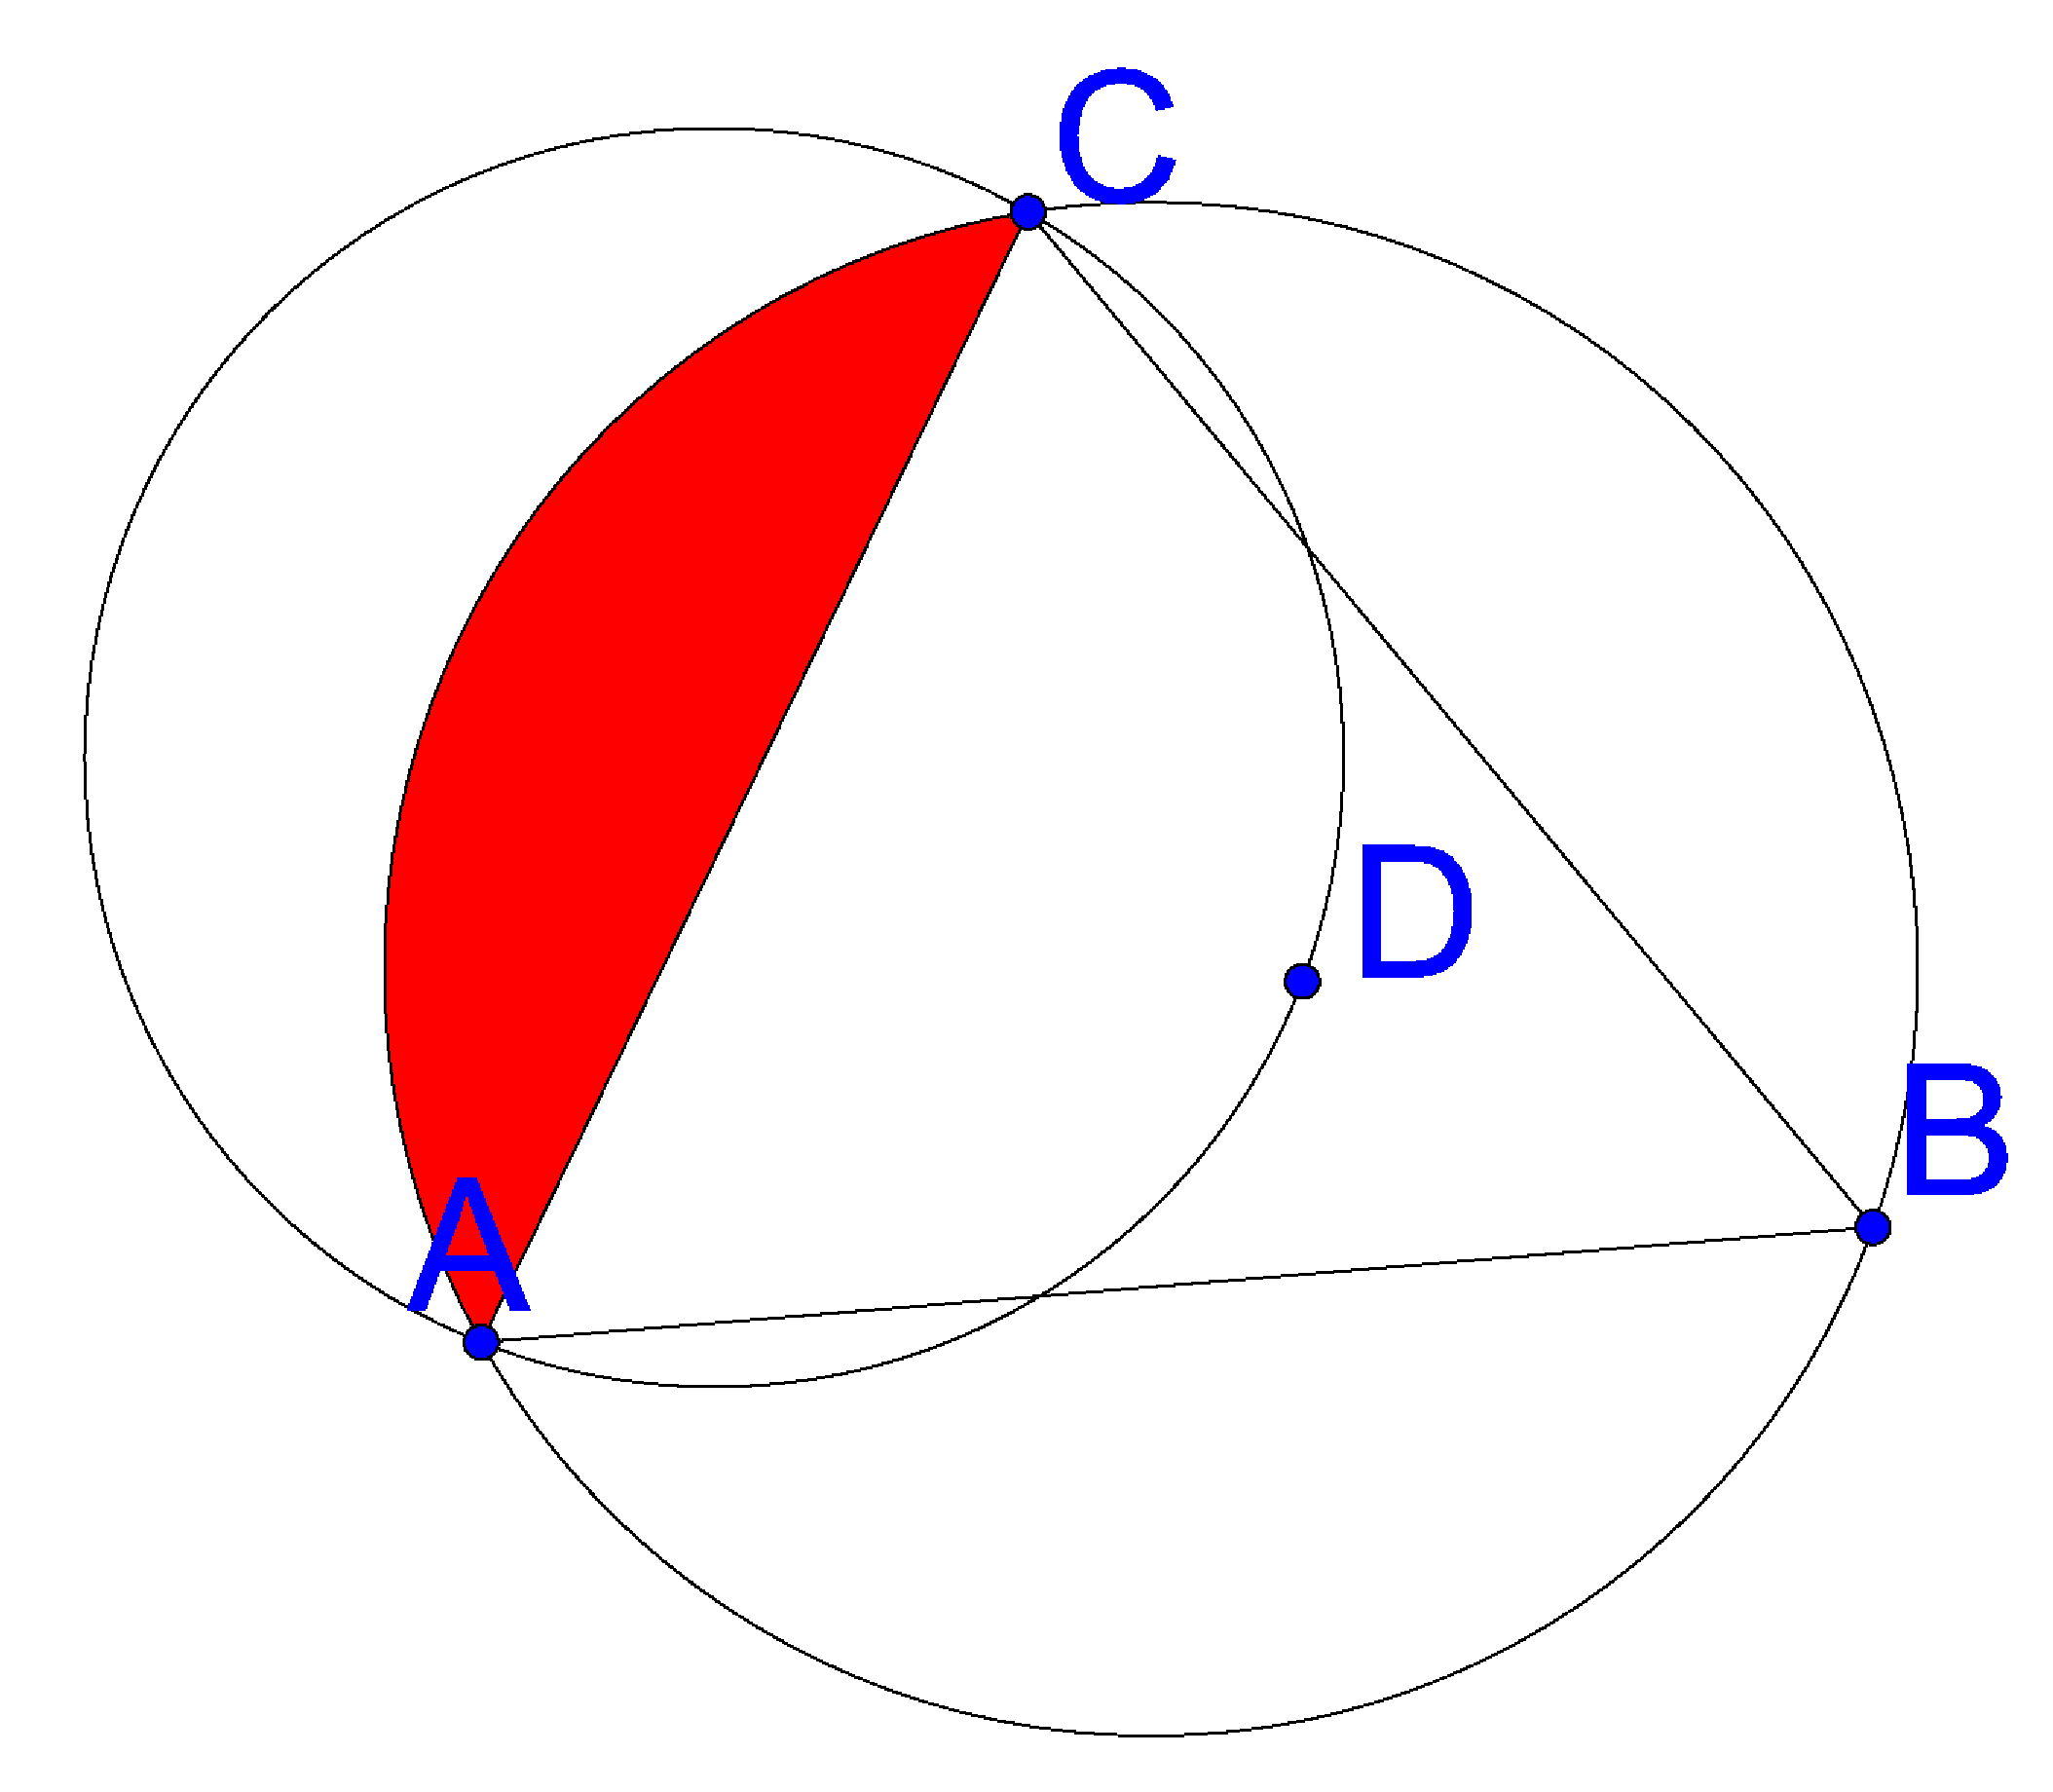
\includegraphics[width=0.2\linewidth]{eps/noPointinRegion.eps}
\caption{The red marked region contains no Points of G because it is always contained in $\bigcirc{ACD} $ which must be empty by definition.}
\label{fig:empty_region}
\end{figure}

Keil and Gutwin \cite{keil} proved the existence of a path between the points $A $ and $B $ and showed that the length of this path is delimited by the length of the arc from $A $ to $B $ on the circle $\bigcirc{ABC} $.
This path connects $A $ and $B $ when no other points of G are inside $\triangle{ABC} $.
The only precondition is that lemma \ref{emptyregion} holds (which it does).
This path is called the \emph{outward path}.
 
First, notice the recursive definition of this path taken from \cite{kanj}:
\begin{enumerate}
\item \textbf{Base case:} If $AB \in G $, the path consists of edge AB.
\item \textbf{Recursive step:} Otherwise, a point must reside in the region $R_3 $ of $(O) $ subtended by chord AB and away from C. 
Let $T $ be such a point with the property that the region of $\bigcirc{ATB} $ subtended by chord $AB $ closer to $T $ is empty. 
We call T an \emph{intermediate point} with respect to the pair of points $(A, B) $.
Let $(O_1) $ be the circle passing through $A $ and $T $ whose center $O_1 $ lies on segment $AO $  and let $(O_2) $ be the circle passing through $B $ and $T $ whose center $O_2 $ lies on segment $BO $.
Then both $(O_1) $ and $(O_2) $ lie inside $(O) $, and $\angle{AO_1T} $ and $\angle{TO_2B} $ are both less than $\angle{AOB} \leq \frac{4\pi}{k} $.
Moreover, the region of $(O_1) $ subtended by chord $BT $ and containing $O_2 $ is empty. Therefore, we can recursively construct a path from $A $ to $T $ and a path from $T $ to $B $, and then concatenate them to obtain a path from A to B.  
\end{enumerate}
Figure \ref{fig:intermediate_point} contains an example for an intermediate point.

The recursive steps assumes $AB \notin G $ and concludes that there must be a point in $R_3 $.
For $G=PDT $ the following lemma proofs the correctness of this assumption:
\begin{lemma}
\label{recursive_step}
For three points $A, B, C \in G $ and $\gamma=\angle{ACB}\leq \frac{2\pi}{k} $ with $k\geq 14 $, $|AB|\leq R $ is satisfied.
\end{lemma} 
\begin{proof}

\begin{equation*}
\begin{split}
  |AB|² &=|BC|²+|AC|² - 2|BC||AC|\cos{\gamma} \\
  &\leq R²+R²   - 2R²\cos{\gamma} \\
  &\leq 2R² - 2R²\cos{\frac{2\pi}{k}}\\
  &\stackrel{a)}{\leq} 2R² - 2R²\cos{\frac{\pi}{7}}\\
  &\stackrel{b)}{\leq} 2R² - 2R²\cdot 0.9 = 0.2R²=\\
  |AB| &\leq \sqrt{0.2} R \leq R
\end{split}
\end{equation*}
In order to minimize $2R²\cos{\frac{2\pi}{k}} $, $\gamma $ must be maximized and hence, it is $\frac{2\pi}{k} $ obtaining a).
Then adjust $\frac{\pi}{7} $ downward to $0.9 $ and receive b).
 
\end{proof}

Lemma \ref{emptyregion} and lemma \ref{recursive_step} proof that there must be a node in $R_3 $, if $AB \notin G $.



\begin{figure}[h!]
\centering
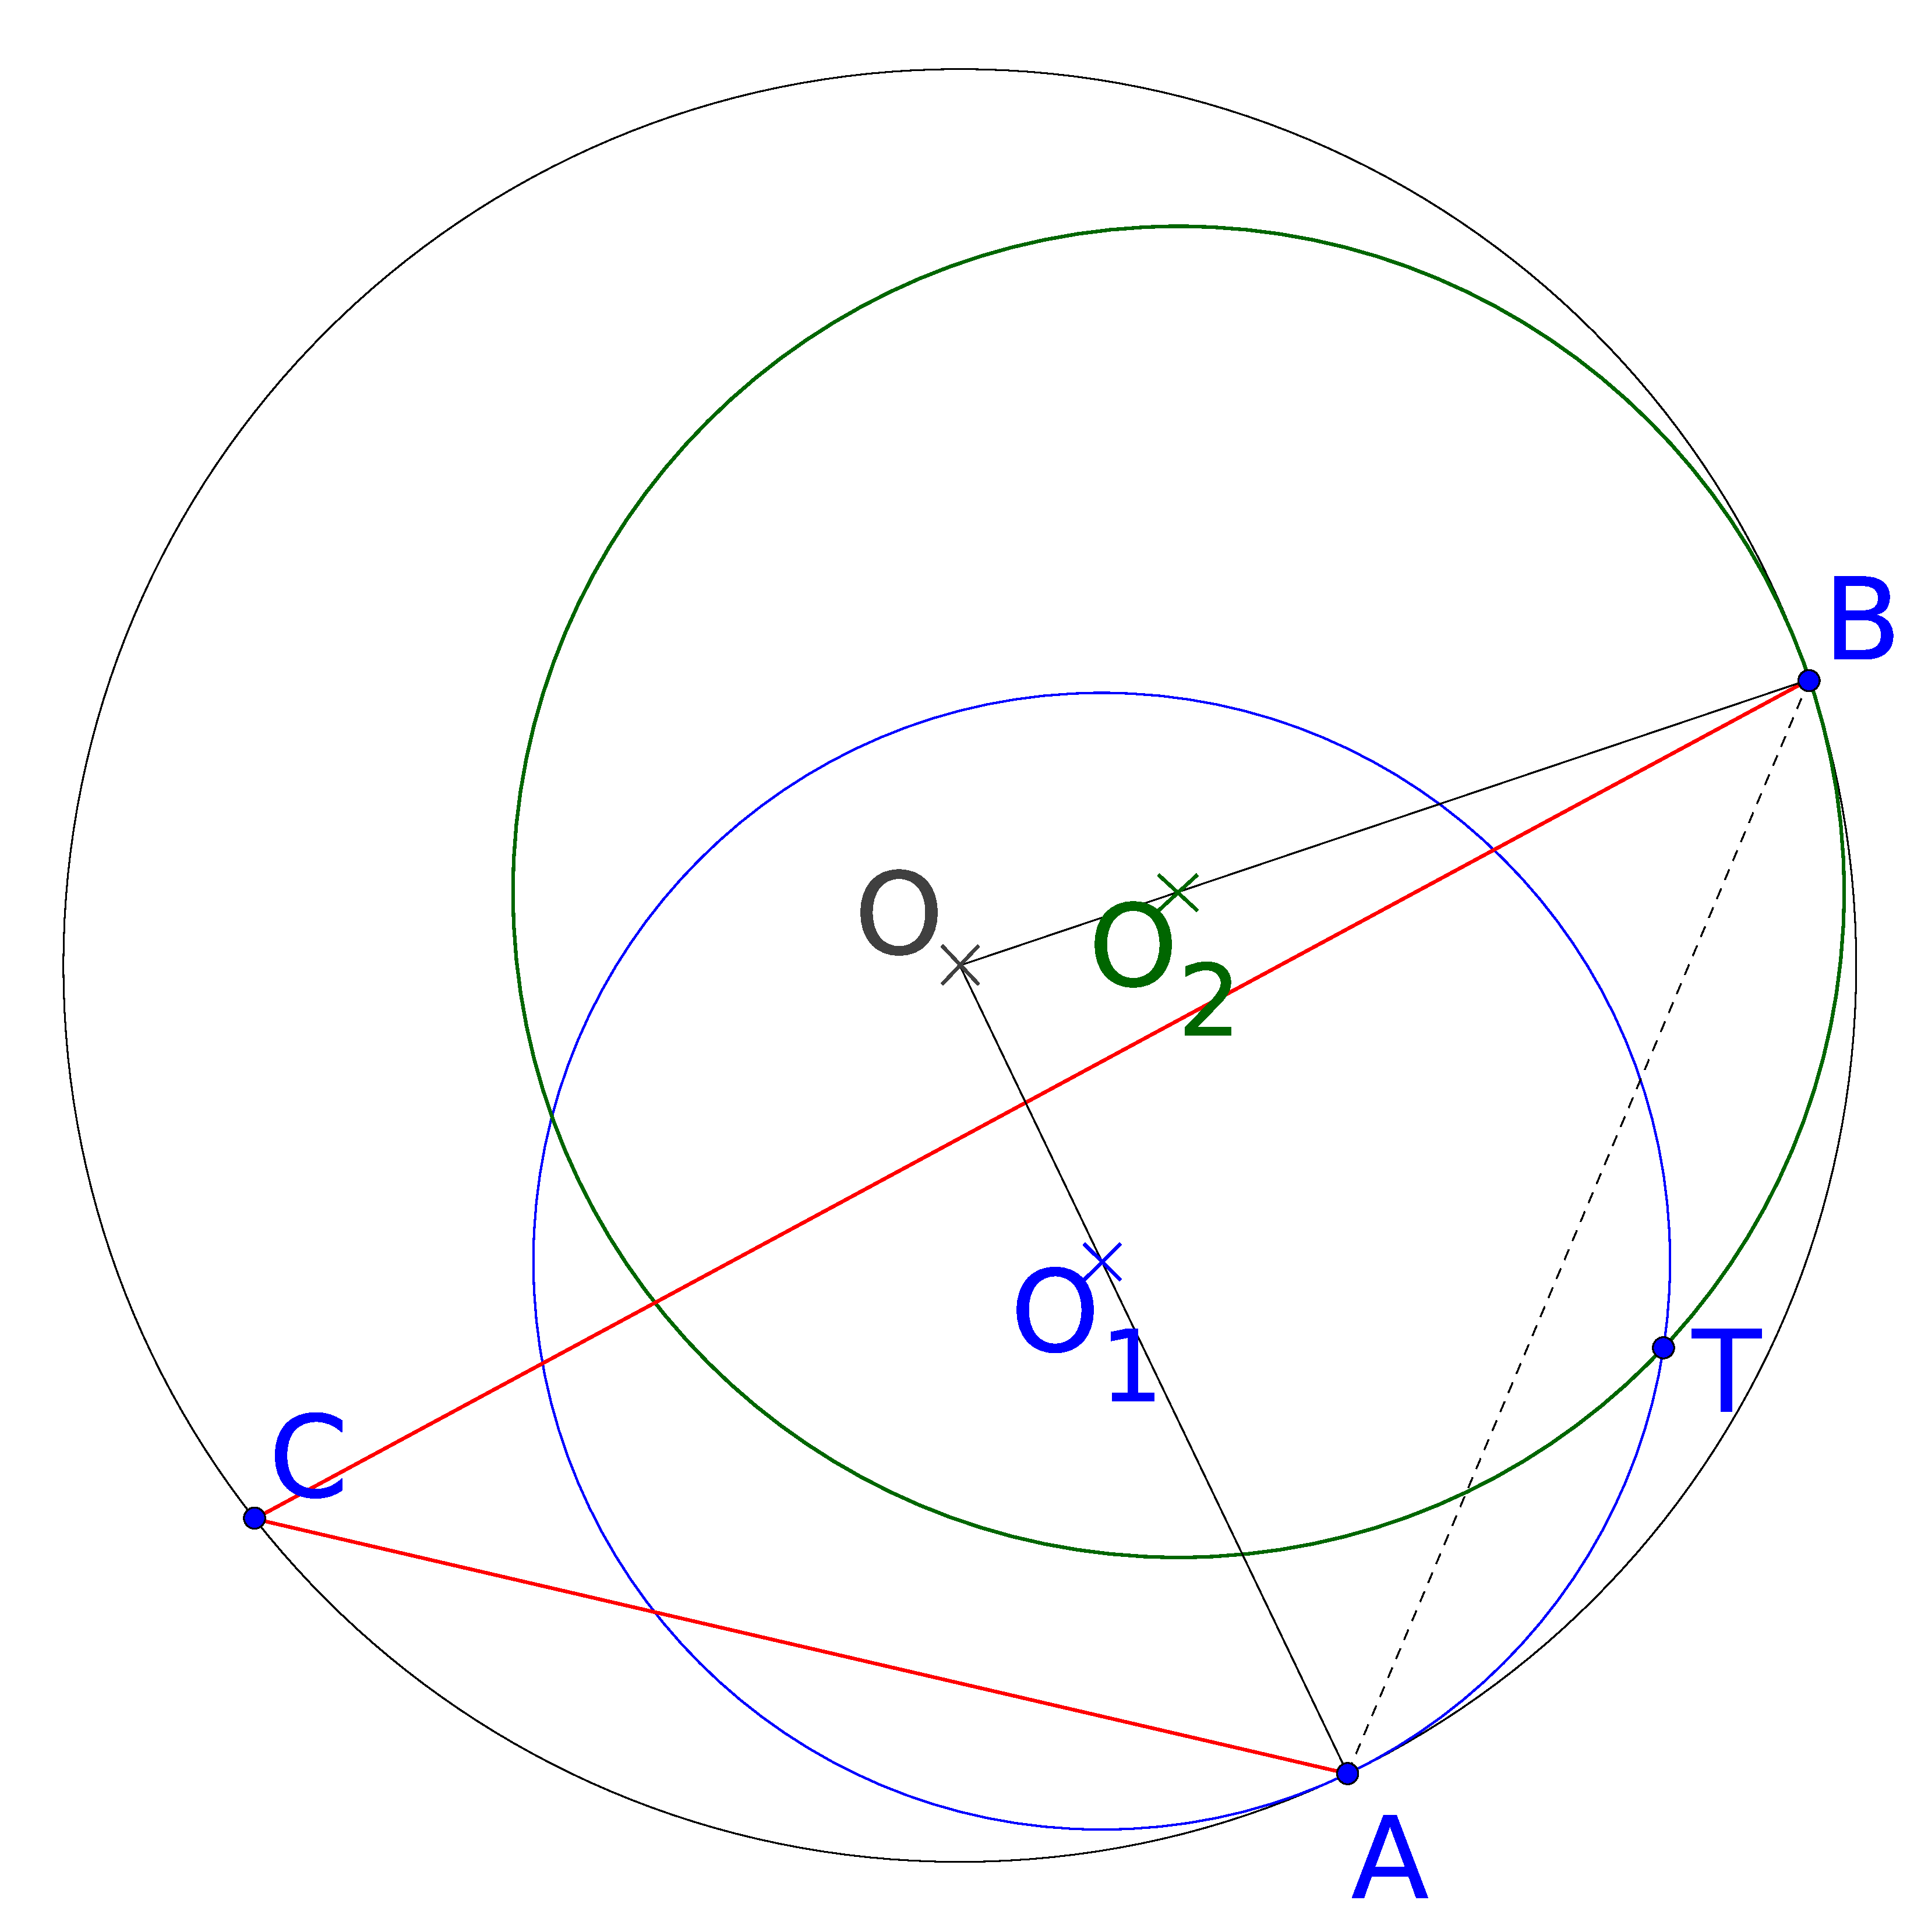
\includegraphics[width=0.5\linewidth]{eps/IntermediatePoint.eps}
\caption{The intermediate point $T $ with respect to pair $(A,B) $, and the circles $O_1 $ and $O_2 $, which are completely within $O $. }
\label{fig:intermediate_point}
\end{figure}


In order to proof proposition \ref{mastertheorem} we need the following proposition (which is from \cite{kanj}):

\begin{prop}
\label{outward_path}
In every recursive step of the outward path construction described above, if $M_p $ is an intermediate point with respect to a pair of points $(M_i, M_j) $, then:
\begin{enumerate}
\renewcommand{\labelenumi}{\alph{enumi})}
\item there is a circle passing through C and $M_p $ that contains no point of G, and
\item circles $\bigcirc{CM_iM_p} $ and $\bigcirc{CM_jM_p} $ contain no points of G, except, possibly, in the region subtended by chords $M_iM_p $ and $M_pM_j $, respectively, away from C.
\end{enumerate}
\end{prop}

\begin{figure}[h!]
\centering
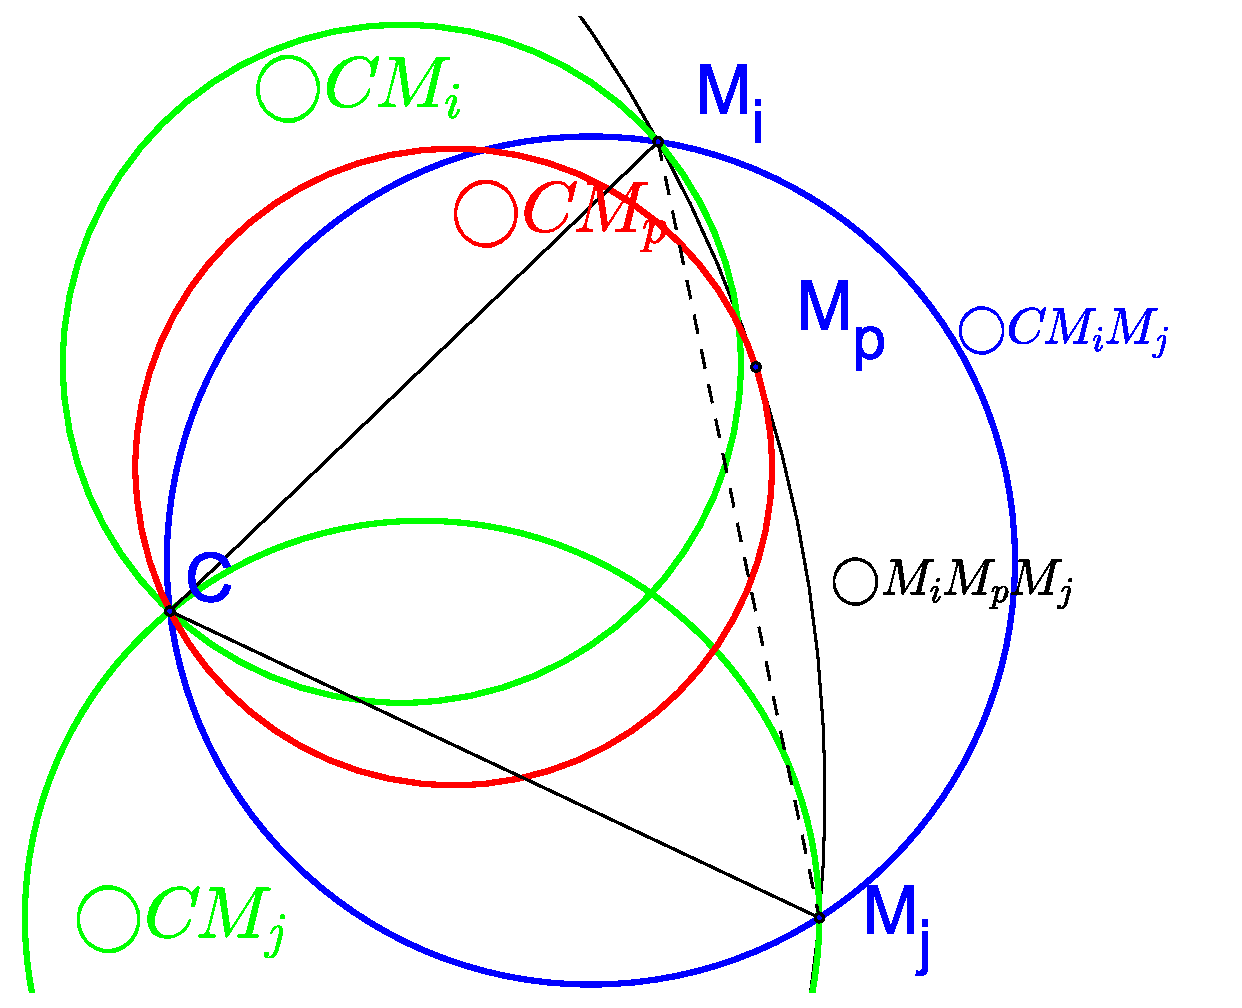
\includegraphics[width=0.9\linewidth]{eps/beweis_outward.eps}
\caption{Example for proof of proposition \ref{outward_path}.}
\label{fig:outward_path_beweis}
\end{figure}

Note that every point $p=1, \cdots, r-1 $, is an intermediate point with respect to a pair $(M_i, M_j) $, where $0\leq i < p <j \leq r  $.
Furthermore, Keil and Gutwin \cite{keil} showed that the length of the path $A =M_0, M_1, \cdots, M_r=B $ is bounded by the length of arc $\overarc{AB} $.
For completeness I copy the proof for proposition \ref{outward_path} from \cite{kanj} with adapted notation.
\begin{proof}

We assume, by induction, that there are circles $\bigcirc{CM_i} $ and $\bigcirc{CM_j} $ passing through $C $ and $M_i $, and $C $ and $M_j $, respectively, containing no points of $G $, and that the circle $\bigcirc{CM_iM_j} $ contains no point of $G $ in the interior of the region $R' $ subtended by chord $M_iM_j $ closer to $C $.
(This is certainly true in the base case because $CA, CB \in G $, by lemma \ref{emptyregion} and by our initial assumptions).

Since $M_iM_j $ is not an edge in $G $, the point $M_p $ chosen in the construction is the point with the property that the region $R $ of $\bigcirc{M_iM_pM_j} $ subtended by chord $M_iM_j $ away from $C $, contains no point of $G $. 
Then the circle passing through $C $ and $M_p $ and tangent to $\bigcirc{M_iM_pM_j} $ at $M_p $ is completely inside $\bigcirc{M_i} \cup \bigcirc{M_j} \cup R \cup R' $, and therefore devoid of points of $G $.
This proves part a).

The region of $\bigcirc{CM_iM_p} $ subtended by chord $M_iM_p $ and containing $C $ is inside $ \bigcirc{M_i} \cup R \cup R' $, and therefore contains no point of $G $ in its interior.
The same is true for the region of $\bigcirc{CM_jM_p} $ subtended by chord $M_jM_p $ and containing $C $, and part b) holds as well.


%Let $G $ be the set of nodes which is created by PDT. 
%Since $CA $ and $CB $ are edges in $G $ there are circles $\bigcirc{CM_i} $ and $\bigcirc{CM_j} $ which have $C $ and $M_i $, and $C $ and $M_j $, respectively, on it's border and do not contain any other nodes of $G $. 
%At this point I assume, without loss of generality, that $M_i $ and $M_j $ lie on the y-axis of the coordinate system and $C $ lies to the left of these points.
%First, notice that $\triangle{CM_iM_j} $ is empty by precondition and the area $R_{\bigcirc{M_iM_pM_j}} $ of $\bigcirc{M_iM_pM_j} $ subtended by chord $M_iM_j $ away from $C $ contains no other points either.
%This proof is divided into three cases.
%\begin{enumerate}
%\item $\bigcirc{CM_p} $ is tangential to $\bigcirc{CM_iM_j} $ at C.
%\item $\bigcirc{CM_p} $ overlaps $\bigcirc{CM_iM_j} $ in the upper halfplane subtended by chord $CM_i $ (away from $M_j $).
%\item $\bigcirc{CM_p} $ overlaps $\bigcirc{CM_iM_j} $ in the lower halfplane subtended by chord $CM_j $ (away from $M_i $).
%\end{enumerate}
%Since the two circles $\bigcirc{CM_p} $ and $\bigcirc{CM_iM_j} $ share the point $C $, $\bigcirc{CM_p} $ cannot overlap $\bigcirc{CM_iM_j} $ on both sides of the edge $CM_p $.
%For case 1 $\bigcirc{CM_p} $ is completely inside $\bigcirc{CM_iM_j} $ and therefore devoid of any points.
%For case 2 $\bigcirc{CM_p} $ is completely inside the area $R_{\bigcirc{M_iM_pM_j}} \cup \bigcirc{CM_iM_j} \bigcirc{CM_i} $ and, therefore, empty.
%$\bigcirc{CM_p} $ cannot overlap $\bigcirc{CM_i} $ because of the following lemma.
%\begin{lemma}
%\label{circles}
%If $A $ and $B $ are points in the plane and are located in different halfplanes of a line $CM_i $, and $A $ and $B $ are not allowed to reside inside a circle $\bigcirc{CM_i} $, there is no circle $\bigcirc{ABC} $ which does not contain $M_i $ and overlaps circle $\bigcirc{CM_i} $.
%\end{lemma}
%\begin{proof}
% Let, without loss of generality, $C $ and $M_i $ be on a line $CM_i $ which is parallel to the y-axis.
%$A $ and $B $ are then located to the left and right of this line.
%You can see this construction in figure \ref{fig:beweis_circles}.
%
%This proof uses a contradiction. % widerspruchsbeweis  -> Florentin fragen
%$A $ cannot reside inside $\bigcirc{CM_i} $, since $CM_i $ is a PDT-edge.
%The circle $c_1 $ must not contain $M_i $ and, therefore, must cross the circle $\bigcirc{CM_i} $ in front of $M_i $.
%Notice that the next part of the circle $c_1 $ must be inside of circle $\bigcirc{CM_i} $, since we started outside.
%Because $c_1 $ must cross $B $ and $B $ lies outside of $\bigcirc{CM_i} $, $c_1 $ crosses a second time $\bigcirc{CM_i} $.
%And the last conclusion is that $C $ is a common point of $\bigcirc{CM_i} $ and $c_1 $.
%Hence, we have got three intersections of $\bigcirc{CM_i} $ and $c_1 $ at least.
%Since $A $ and $B $ lie outside of $\bigcirc{CM_i} $, these two circles are not equal.
%But two circles which intersect at least three times and are not equal, do not exist.
%\end{proof}
%The proof of case 3 works analogously.
%These conclusions proof part a) of proposition \ref{outward_path}.
%
%The following part of this work proofs part b) of the same proposition.
%The main argument of this proof is that $\bigcirc{CM_iM_p} $ is contained completely in the area $\bigcirc{CM_i} \cup  R_{\bigcirc{M_iM_pM_j}} \cup R2_{\bigcirc{CM_iM_j}} $ with $R2_{\bigcirc{CM_iM_j}} $ being the area of $\bigcirc{CM_iM_j} $ subtended by chord $M_iM_j $ closer to $C $.
%I show that every possible position of $\bigcirc{CM_i} $ includes the area $R3_{\bigcirc{CM_iM_p}} $ of $\bigcirc{CM_iM_p} $ subtended by chord $CM_i $ away from $M_j $.
%The proof is divided into three cases of how $\bigcirc{CM_i} $ can be located:
%\begin{enumerate}
%\item $\bigcirc{CM_i} $ is equal to $\bigcirc{CM_iM_p} $.
%\item $\bigcirc{CM_i} $ overlaps $\bigcirc{CM_iM_p} $ in the halfplane subtended from line $CM_i $ away from $M_j $.
%\item $\bigcirc{CM_i} $ overlaps $\bigcirc{CM_iM_p} $ in the halfplane subtended from line $CM_i $ closer to $M_j $.
%\end{enumerate}
%First, assume, without loss of generality, that $C $ and $M_i $ lie on a horizontal line and $M_j $ is located below this line.
%$\bigcirc{CM_iM_p} $ can only overlap $\bigcirc{CM_i} $ on one side of line $CM_i $, since they share these two points.
%
%For case 1, since $\bigcirc{CM_i} $ is empty, $\bigcirc{CM_iM_p} $ must be empty, too.
%
%For case 2, $\bigcirc{CM_i} $ moves up, away from $M_j $, expanding the area in the same direction of which $R3_{\bigcirc{CM_iM_p}} $ is located.
%So, $R3_{\bigcirc{CM_iM_p}} $ cannot overlap $\bigcirc{CM_i} $ in this case.
%
%Case 3, the only case where $R3_{\bigcirc{CM_iM_p}} $ would overlap $\bigcirc{CM_i} $, cannot occur, since $M_p \in G $ and $M_p $ is, obviously, located on $\bigcirc{CM_iM_p} $.
%So, if $\bigcirc{CM_i} $ moves down, towards $M_j $, it would contain $M_p $, which cannot happen, since $\bigcirc{CM_i} $ is a PDT-circle. 
%
%Notice that the proof for $\bigcirc{CM_jM_p} $ works analogously substituting $M_i $ with $M_j $ and vice versa.
 
\end{proof}
\begin{figure}[h!]
\centering
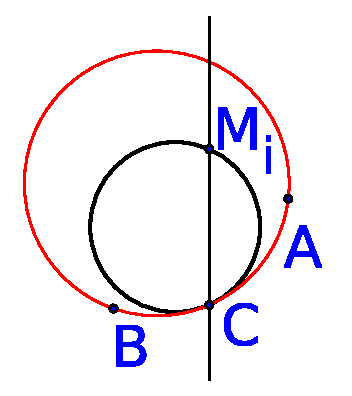
\includegraphics[width=0.5\linewidth]{eps/beweis_circles.eps}
\caption{Example of the construction of lemma \ref{circles}.}
\label{fig:beweis_circles}
\end{figure}
Another fact we need in order to proof proposition \ref{mastertheorem} is the following:
\begin{fact}
\label{outward_3}
If four points $A $, $B $, $C $ and $M_1 $ are on one circle and $C $ and $M_1 $ are on different halfplanes of chord $AB $, then $\angle{AM_1B} + \angle{ACB} =\pi $ is true (please refer to figure \ref{fig:winkel_fuer_outward_3} for an graphical illustration of this lemma).\footnote{see Euklid, book 3, proposition 22, for proof}
\end{fact}

\begin{figure}[h!]
\centering
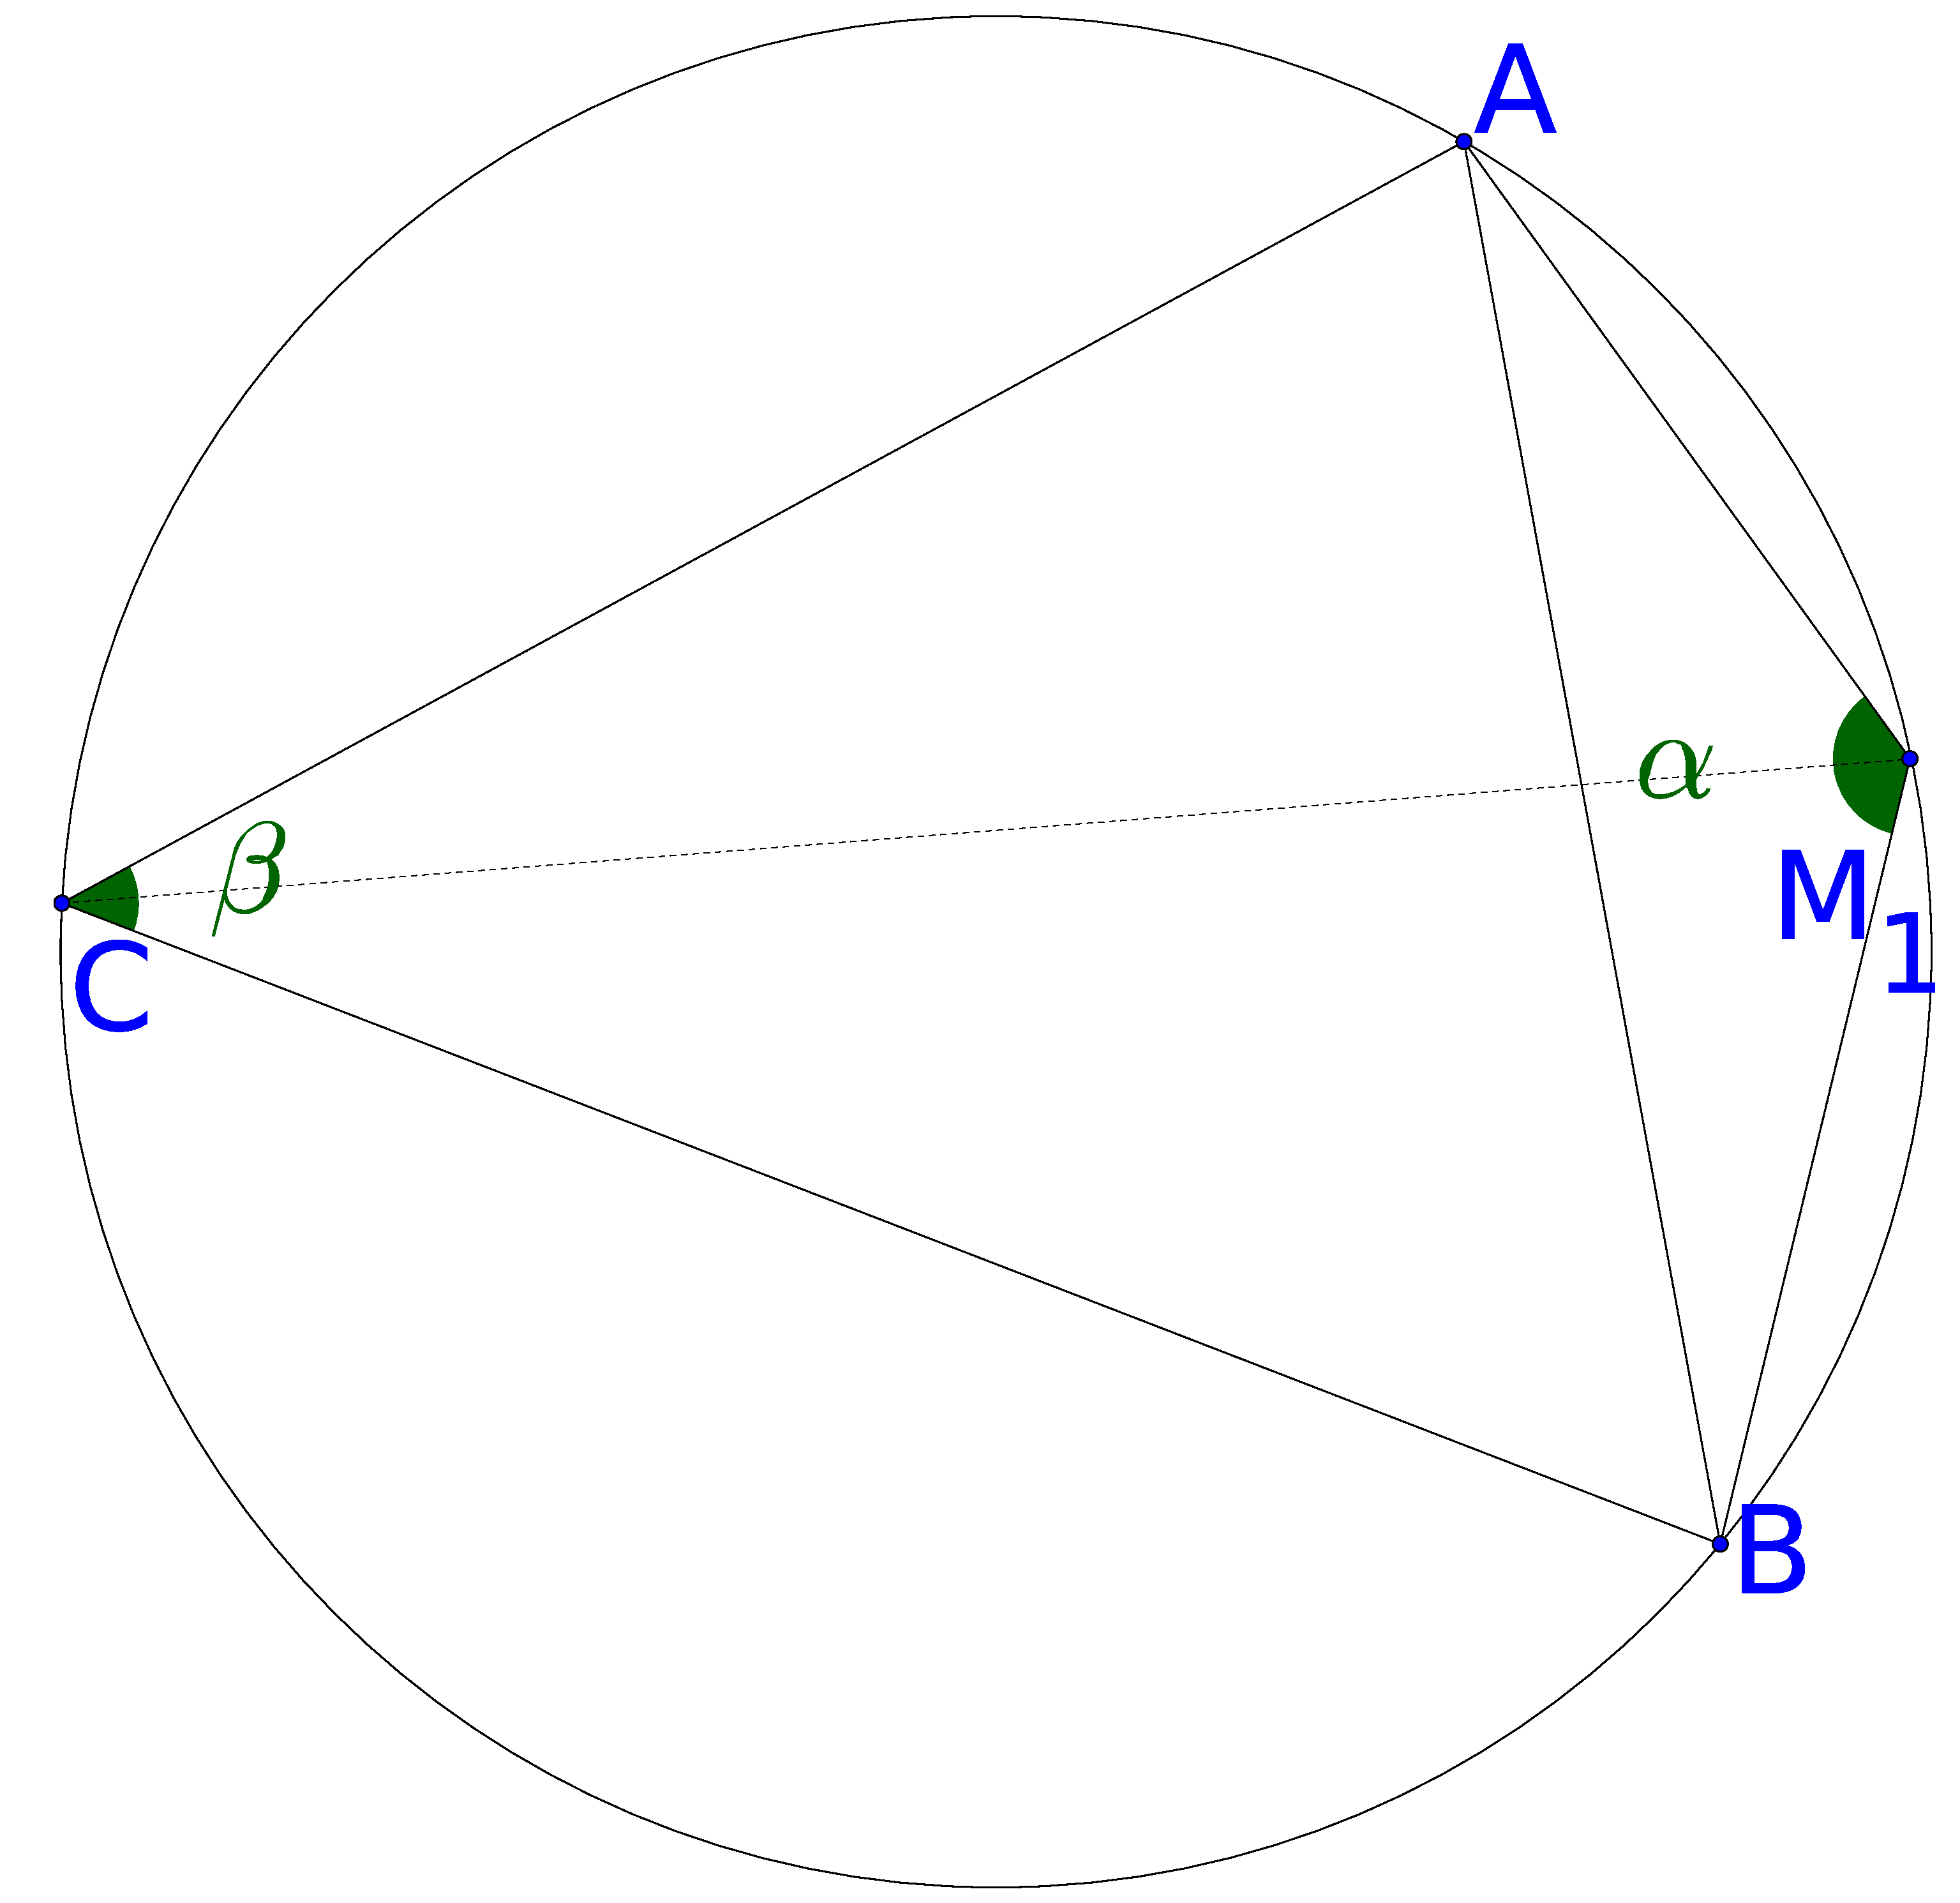
\includegraphics[width=0.4\linewidth]{eps/Winkel_fuer_outward_3.eps}
\caption{Example for lemma \ref{outward_3} }
\label{fig:winkel_fuer_outward_3}
\end{figure}

Now, we can proof the following lemma from \cite{kanj}, which shows, that for the case of the outward path, proposition \ref{mastertheorem} is satisfied:

\begin{lemma}
Let $k \geq 14$ be an integer, and let $CA $ and $CB $ be edges in $G $ such that $\angle{BCA} \leq \frac{2\pi}{k} $ and $CA $ is the shortest edge in the angular sector $\angle{BCA} $. There exists a path $p : A=M_0, M_1, \dotsc, M_r=B $ in $G $ such that:
\begin{enumerate}
\renewcommand{\labelenumi}{(\roman{enumi})}
\item $|CA| + \sum_{i=0}^{r-1}|M_iM_{i+1}| \leq (1+2\pi(k \cos(\frac{\pi}{k}))^{-1})|CB|$
\item There is no edge in $G $ between any pair $M_i $ and $M_j $ lying in the closed region delimited by $CA, CB $ and the edges of $p $, for any $i $ and $j $ satisfying $0 \leq i < j -1 \leq r $.
\item $\angle{M_{i-1}M_iM_{i+1}} > \pi - \frac{2\pi}{k} $, for $i=1,\dotsc,r-1 $.
\item $\angle{CAM_1} \geq \frac{\pi}{2} - \frac{pi}{k} $.
\end{enumerate}	 
\end{lemma}

\begin{proof}
This proof is performed almost equal to \cite{kanj}, but covering more details.
%and $\sin{\theta} = \frac{|AB|}{2|OA|}) $
\renewcommand{\labelenumi}{(\roman{enumi})}%
\begin{enumerate}
\item 
\begin{equation*}
\begin{split}
|CA|+|\overarc{AB}| &= |CB| + 2\theta \cdot |OA| \\
&\stackrel{a)}{=}|CB| + (\frac{\theta}{\sin{\theta}})\cdot |AB| \\
&\stackrel{b)}{=} |CB| + (\frac{\theta}{\cos{\frac{\theta}{2}}}) \cdot |CB|\\
&\stackrel{c)}{\leq} (1+2\pi(k \cos{\frac{\pi}{k}})^{-1}) |CB|  
\end{split}
\end{equation*}
In \cite{keil} Keil and Gutwin proved that the length of the path between $A $ and $B $ is bounded by $|\overarc{AB}|$ and thus, it suffices to show that $|CA| + |\overarc{AB}|\leq (1+2\pi(k \cos{\frac{\pi}{k}})^{-1})$.
Since $|CA| \leq |CB| $, $|CA|+|\overarc{AB}| $ is largest, when $CA $ and $CB $ are symmetrical to the diameter of $\bigcirc{ABC} $, we can assume $|CA|=|CB| $.
$|\overarc{AB}| $ can be replaced with $2\theta \cdot |OA| $ (angle times radius).
For every chord $s $ of a circle $(c) $ it is true, that $s=2r\sin{\frac{\alpha}{2}} $, with $r $ being the radius of $(c) $ and $\alpha $ being the angle between the endpoints of $s $ in middlepoint $c $ facing $s $.
Note that $\alpha = 2\theta $. 
These equations proof a).

Next, substitute $|AB| $ with $|AB| = \sin{\frac{\theta}{2}} \cdot 2|CB| $ and replace $\sin{\theta} $ with the trigonometry identity $\sin{\theta}=2\sin{\frac{\theta}{2}} \cos{\frac{\theta}{2}} $.
You receive equation b).

At last, substitute $\theta $ using inequality $\theta \leq \frac{2\pi}{k} $ with $k > 2 $, obtaining c).

\item  Suppose, $M_i $ and $M_j $ is an edge in $G $, then there exists a circle with these two points on it's border which does not contain any other node of $G $.
So, $M_p $ must lie outside of this circle.
By proposition \ref{outward_path} part a) there is a circle $\bigcirc{CM_p} $ trough $C $ and $M_p $ which is empty.
These two last observations contradict each other, since $\bigcirc{M_iM_j} $ would always contain $M_p $.
If $M_p $ does not reside in the circle $\bigcirc{M_iM_j} $, this circle and the circle $\bigcirc{CM_p} $ would cross at least three times (and are not equal), which cannot exist.

\item Since the angles $\alpha $ and $\beta $ between opposite points of a chord in a rectangle which corners lie on a circle are supplementary, this is a fact: $\angle{AM_1B}=\pi - \angle{ACB} $ (see lemma \ref{outward_3} for more details).
The angle $\angle{M_{i-1}CM_{i+1}} $ is smallest, if $M_{i-1} $ and $M_{i+1} $ lie on the circle. 
Note, by precondition we assume $\angle{BCA} \leq \frac{2\pi}{k} $.
These facts proof following inequalities:
\begin{equation*}
\begin{split}
 \angle{M_{i-1}M_iM_{i+1}}&\geq \pi - \angle{M_{i-1}CM_{i+1}}\\
 &\geq \pi - \angle{BCA} \\ &\geq \pi - \frac{2\pi}{k}\\
\end{split}
\end{equation*}



 %http://www.regentsprep.org/regents/math/geometry/gp15/circleangles.htm
\item Since $M_1 $ is inside the area subtended by chord $AB $ from $\bigcirc{ABC} $ \emph{away} from $C $, it is true that $\angle{CAM_1} \geq \angle{CAB} \geq \frac{\pi}{2} -\frac{\pi}{k} $.
The last inequality is true because:
 \begin{equation*}
  \begin{split}
   \angle{CAB}+\angle{ABC}+\underbrace{\angle{BCA}}_{\leq \frac{2\pi}{k}}&=\pi\\
   \angle{CAB}+\angle{ABC} &\geq \pi - \frac{2\pi}{k} \\
   \angle{CAB} &\geq \frac{\pi-\frac{2\pi}{k}}{2}=\frac{\pi}{2}-\frac{\pi}{k}
   \end{split} 
\end{equation*}
Since $CA \leq CB $, $\angle{CAB} $ can be at most the half of $\pi - \frac{2\pi}{k} $, proving the last inequality.

\end{enumerate}
\end{proof}

 
%\begin{figure}[h!]
%\centering
%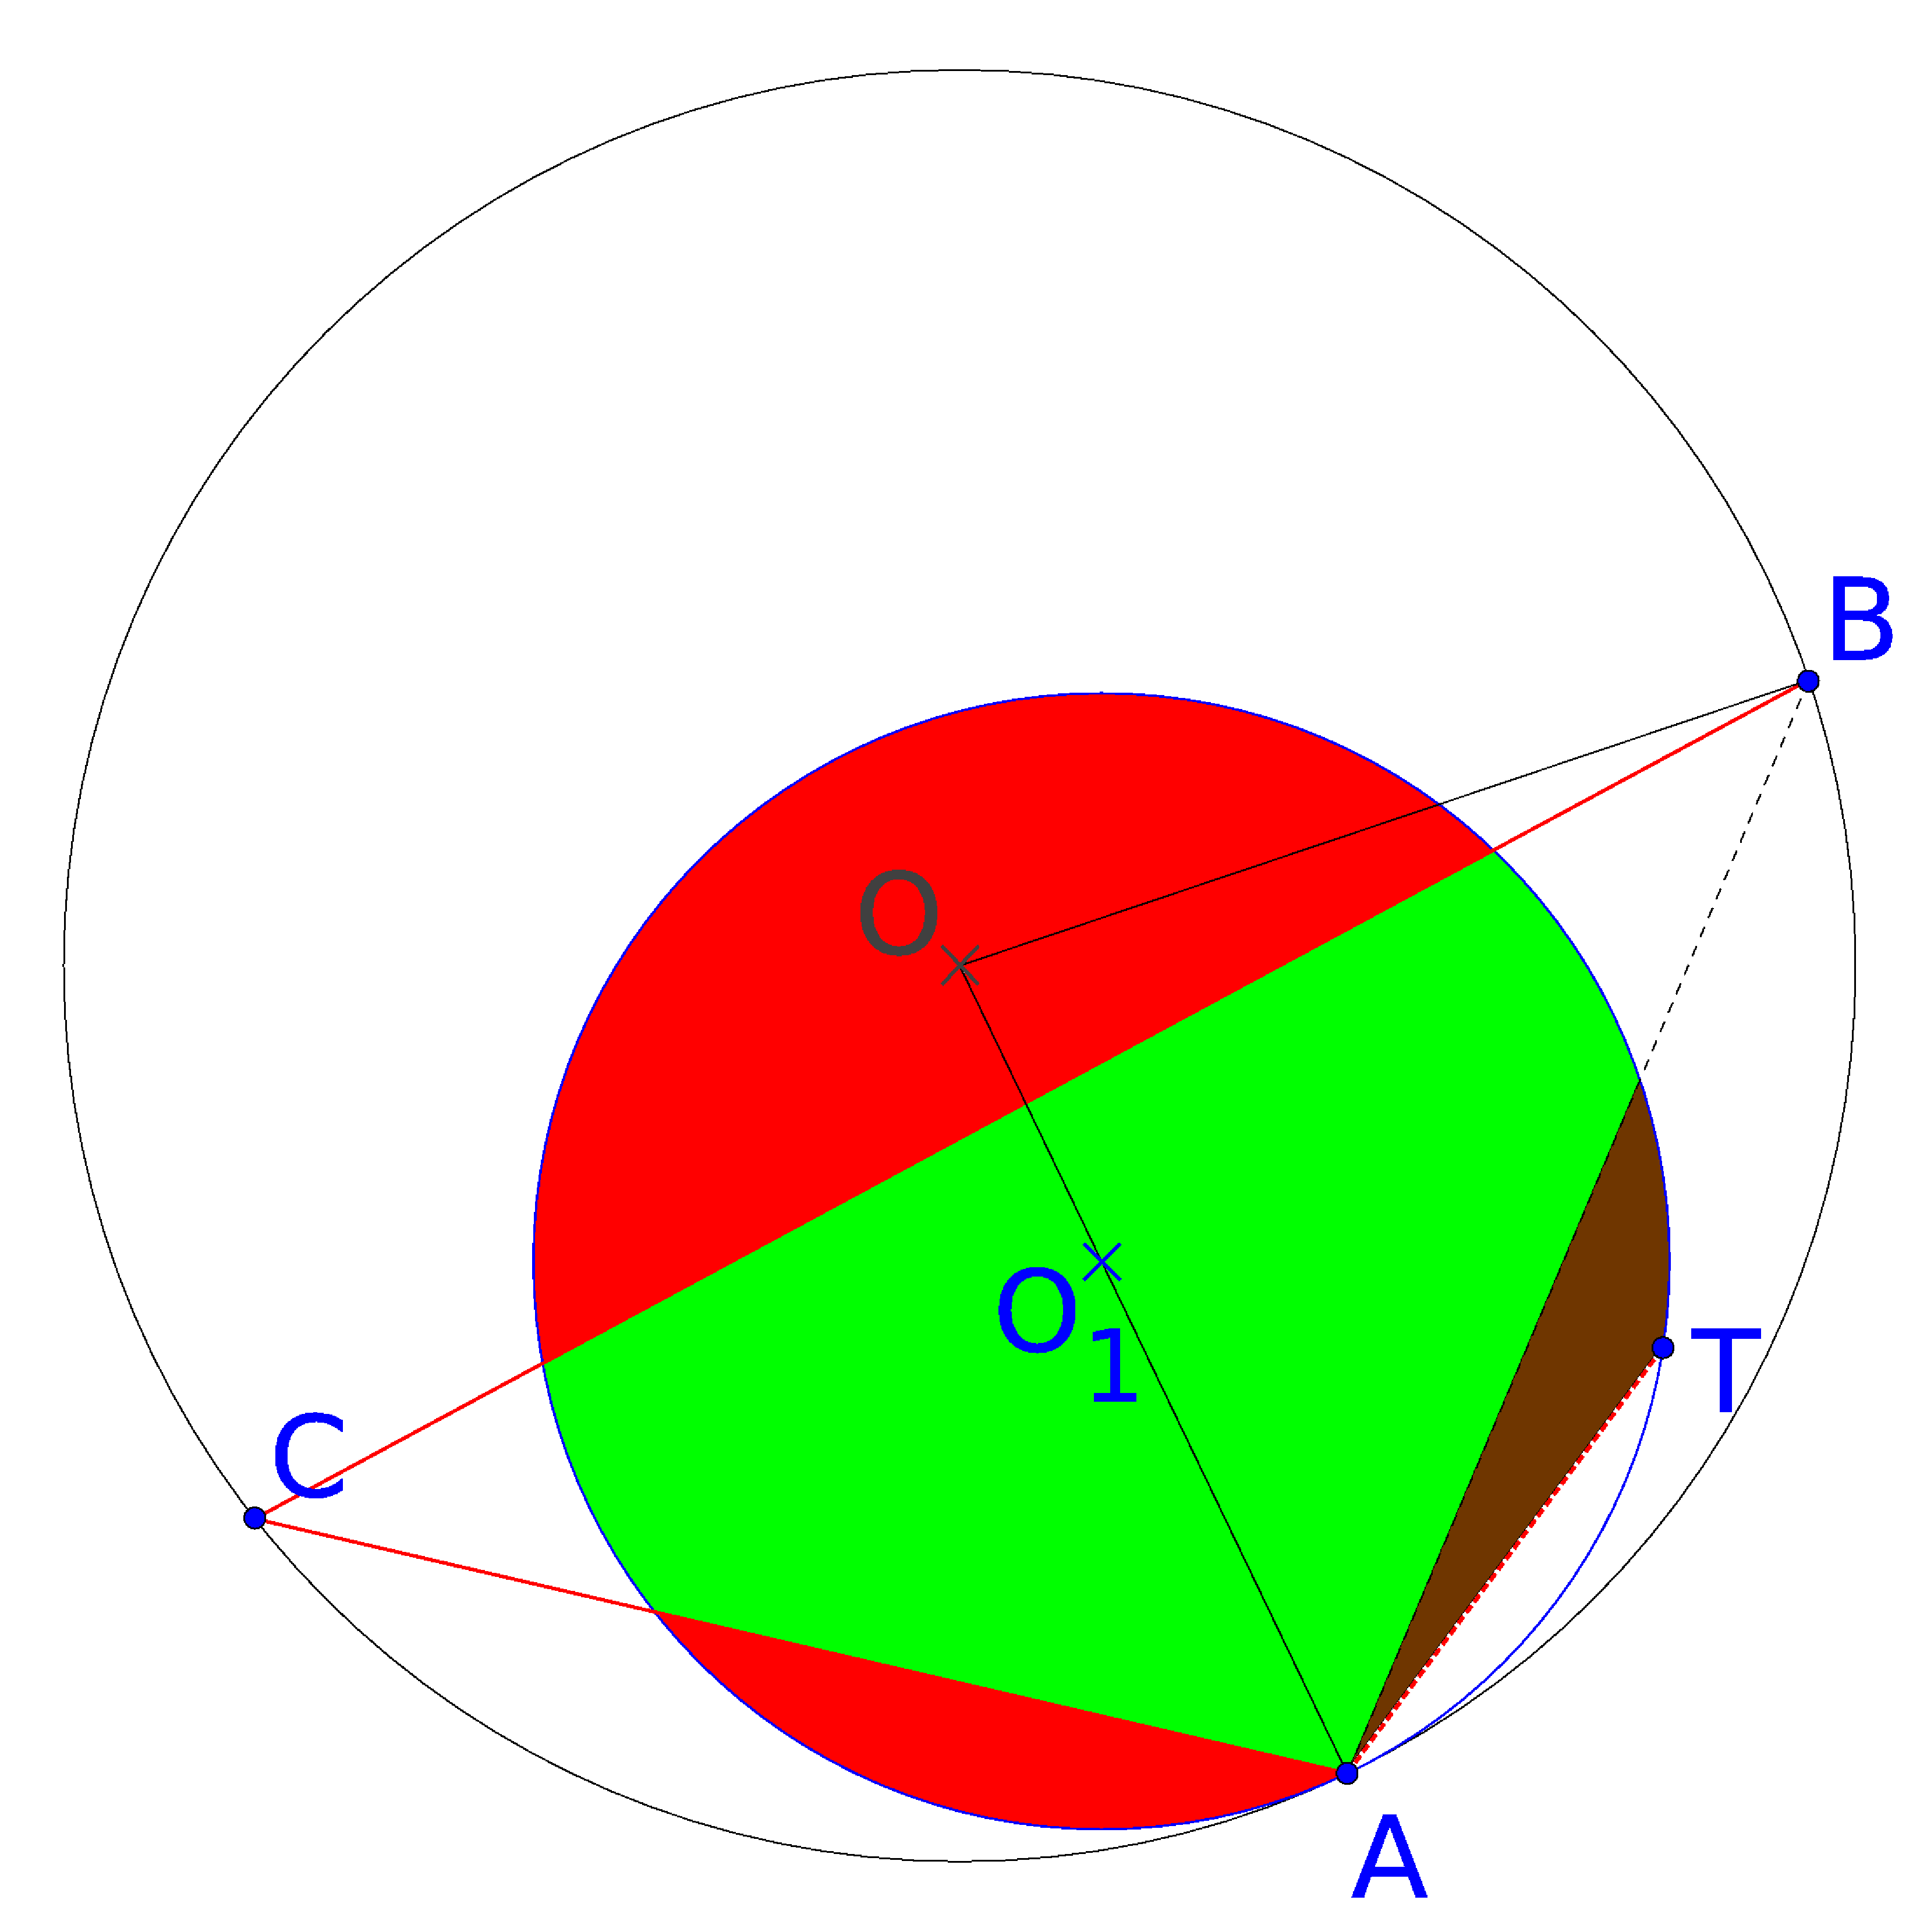
\includegraphics[width=0.5\linewidth]{eps/IntermediatePoint_beweis.eps}
%\caption{The red regions must be empty by lemma \ref{emptyregion}, the green area is empty by precondition and the brown region must be empty by ... }
%\label{fig:intermediate_point_beweis}
%\end{figure}
%
%
%\begin{enumerate}
%\item $|CA| + \sum\nolimits_{i=0}^{r-1} |M_iM_{i+1}| \leq (1+2\pi (k*\cos{\frac{\pi}{k}})^{-1})|CB| $
%\item There is no edge in G between any pair $M_i $ and $M_j $ lying in the closed region delimited by CA, CB and the edges of p, for any i and j satisfying $0 \leq i < j-1 \leq r $ 
%\item $\angle{M_{i-1}M_iM_{i+1}} > \frac{k-2}{k}\pi $, for $i=1, ..., r-1 $ 
%\item $\angle{CAM_1} \geq \frac{\pi}{2}-\frac{\pi}{k} $
%\end{enumerate}




\subsection{inward Path}
Now, we perform the proof for the case when $\triangle{ABC} $ contains other nodes.

Let $S $ be the set of points which contains points $A $ and $B $, and all the points interior to $\triangle{ABC} $ excluding $C $.
Then $CH(S) $ are all the points which are on the convex hull of $S $.
Let these points be called $N_0=A $ and $N_t=B $ and points $N_1 , \cdots ,N_{t-1} $ are the points on $CH(S) $ which lie inside $\triangle{ABC} $. 
The following proposition is taken from \cite{kanj}:
\begin{prop}
\label{inward_pre}
\begin{enumerate}
\renewcommand{\labelenumi}{\alph{enumi})}
The following are true:
\item for every $i =0,\cdots,s-1: $ $|CN_i| \leq |CN_{i+1}| $, and
\item for every $i=0, \cdots, s-2: $  $\angle{N_{i}N_{i+1}N_{i+2}} \geq \pi $, where $\angle{N_{i}N_{i+1}N_{i+2}} $ is the angle facing point $C $.
\end{enumerate} 
\end{prop}
\begin{proof}
Since $CA $ is the shortest edge in the angular sector $\angle{BCA} $, $|CA| \leq CN_i $, for $i=1 ,\cdots, t-1 $  and since $N_1 , \cdots, N_t $ are on $CH(S) $, a) is true.

Part b) follows from the convexity of $CH(S) $. All interior angles to $CH(S) $ measure at most $\pi $, so all the exterior angles fulfil $\angle{N_{i-1}N_iN_{i+1}}\geq \pi $ 
\end{proof}

Since $CN_i \leq CN_{i+1} $ and no other point of $G $ lies inside $\triangle{N_iCN_{i+1}} $, $CN_i $ is the shortest edge in the angular sector $\angle{N_iCN_{i+1}} $.
%related work: kanj hat neues ergebnis mit knotenbeschränkung kleiner gleich 11...
%improved local algorithms   2012
\section{Conclusio}
RMYS is due to its reactivity a robust algorithm to construct a bounded degree, planar graph which is most likely an Euclidean spanner.
As for now, it is not appropriate to use it to create a local view on just one node in consequence of the message overhead it creates.
However, it is well suited to create a complete graph in a reactive way while providing a constant node degree on top of planarity and a constant spanning ratio.
RMYS is the first algorithm which inherits all these graph properties and is created in a reactive way.

For the past years reactivity in ad hoc sensor networks reduced permanently the message overhead to create planar graphs which later turned out to be spanners.
In addition, it is now possible to append the property of a constant node degree for each node in the graph to reactive approaches.
This saves additional messages if a routing protocol uses the underlying RMYS graph.

In order to minimize the constant node degree bound of $14 $ further research should focus on formally proving the spanning ratio of RMYS and check whether it is possible to lower the degree bound without increasing the spanning ratio significantly.
Another interesting point for future research is to reduce the message overhead for RMYS when it is executed on one node.
For instance, under the condition that all possibilities where RMYS creates a uni directional edge are known one can possibly omit the last broadcast completely.
Instead, one must find a pattern for each of these possibilities to detect uni directional edges without sending additional messages (REF GEBIET).
\include{Programming}

\begin{appendix}
%% include your appendices here
%\include{appendix-A}
\end{appendix}
%%%%%%%%%%%%%%%%%%%%%%%%%%%%%%%%%%%%%%%%%%%%%%%%%%%%%%%%%%%%%%%%%
%%%%%%%%%%%%%%%%%%%%%%%%%%%%%%%%%%%%%%%%%%%%%%%%%%%%%%%%%%%%%%%%%
%\addcontentsline{toc}{chapter}{Bibliography}
\bibliographystyle{unsrt}
\bibliography{db-refs,local-refs}
\end{document}
%%%%%%%%%%%%%%%%%%%%%%%%%%%%%%%%%%%%%%%%%%%%%%%%%%%%%%%%%%%%%%%%%
%%%%%%%%%%%%%%%%%%%%%%%%%%%%%%%%%%%%%%%%%%%%%%%%%%%%%%%%%%%%%%%%%
\endinput
%%
%% End
